\section{Formalization}
\begin{definition}A directed graph $G = \{V, Ed\}$ consists of a finite set $V$ of vertexes, and a set $Ed$ of edges. An edge connects a source vertex to a target vertex. The source and target vertexes of an edge ed are obtained by $src(ed)$ and $tgt(ed)$.
\end{definition}

\begin{definition}A UML vertex v $\in$ V has a kind $v.kind \in$  \ti{\{initial, final, state, composite, concurrent, join, fork, choice, junction, enpoint, expoint, history\}}. Each vertex $v$ has a name and we write $v.name$. 
\end{definition} 

\begin{definition}A region $r \in \mathcal{R}$ is composed of one or several vertexes, and contained by a state $s$: $ctner(r) = s$. 
\end{definition}	

\begin{definition} A UML state s is a vertex v where v.kind $\in$ {state, composite, concurrent}. s has an $entry$, an $exit$ and a $doActivity$ action. A composite state cs contains one or more vertexes. We write subvertexes(cs) is a set of vertexes contained by cs and $ctner(v)$ refers to the containing state of the vertex v. A concurrent state contains more than one region.
\end{definition}		

\begin{definition} An action $act$ $\in$ $ActLang$ is a set of statements written in an object-oriented programming language $ActLang$. A guard is a boolean expression written in $ActLang$.
\end{definition}

\begin{definition} A transition $t \in T$ is an edge connecting two vertexes. A transition has a guard $guard(t)$, an effect $effect(t)$, and is associated with a set of events $\subset$ E. We write events(t) as the associated set of events. A transition has a type $t.type$ $\in \{trigger, triggerless, guardless\}$ and a kind $t.kind \in {external, local, internal}$.
\end{definition}

\begin{definition} A \ti{TimeEvent} $te$ an internal event and specifies the time of occurrence $d$ relative to a starting time. The latter is specified when a state, which accepts the time event, is entered. 
\end{definition}

\begin{definition} A \ti{Signal} $sig$ contains data. 
\end{definition}

\begin{definition} A \ti{SignalEvent} $se$ is associated with a signal $sig$ and is occurred if $sig$ is received by a component, which is an active UML class. 
\end{definition}	

\begin{definition}
	A \ti{ChangeEvent} $che$ is associated with a boolean expression $ex(che)$ written in $ActLang$. $che$ is emitted if $ex(che)$ changes from true(false) to false(true).
\end{definition}

\begin{definition}
	A \ti{CallEvent} $ce$ is associated with an operation $op(ce)$. $ce$ is emitted if there is a call to $op(ce)$.
\end{definition}

Suppose that for each vertex \ti{v} $\in$ $V$, its incoming and outgoing transition lists are extracted by the functions $incomings$ and $outgoings$, respectively. For a list $l$, the function $head$ is used to get the first element of the list. If $v.kind = concurrent$, suppose $regions(v)$ is the region set contained by $v$. Given a transition t:
\begin{itemize}
	\item $t.type = trigger$ if $\#events(t) > 0$.
	\item $t.type = triggerless$ if $\#events(t) = 0$.
	\item $t.type = guardless$ if $(guard(t) = true \vee \nexists guard(t)$.
	\item $t.type = triggerguardless$ if $\#events(t) = 0 \wedge (guard(t) = true \vee \nexists guard(t))$.
\end{itemize}

The behavior of an active class $C$ is described by using a state machine whose definition is as following:	

\begin{definition} A state machine sm is a graph specified by $\{V, T\}$ associated with a set of events $E$. A state machine is a special composite state which has no incoming and no outgoing transitions. A root vertex $v$ is a direct sub-vertex of the state machine, $ctner(v) = sm$. The set of regions contained by $sm$ is written $\mathcal{R}$.
\end{definition}	

For each vertex $v$ $\in$ $V$, we write the following sets $T_{ins} (v) = incomings(v), T_{outs}(v) = outgoings(v)$, $t_{first} = head(t_{outs})$; transitive transition sets $T_{ins}^{+}$ and $T_{outs}^{+}$: 
\begin{strip}
	\begin{equation}
	T_{ins}^{+} (v) =    \left\{
	\begin{array}{ll}
	T_{ins}(v) & v.kind \notin \{composite, concurrent\}  \\
	T_{ins}(v) \cup \bigcup\limits_{sub \in subvertexes(v)} T_{ins}^{+} (sub) & v.kind \in \{composite, concurrent\} \\
	\end{array} 
	\right.
	\end{equation}
	
	\begin{equation}
	T_{outs}^{+} (v) =    \left\{
	\begin{array}{ll}
	T_{outs}(v) & v.kind \notin \{composite, concurrent\}  \\
	T_{outs}(v) \cup \bigcup\limits_{sub \in subvertexes(v)} T_{outs}^{+} (sub) & v.kind \in \{composite, concurrent\} \\
	\end{array} 
	\right. 
	\end{equation}
\end{strip}

\begin{definition} Transitive container $ctner^+(v)$ of a vertex $v$ of a state machine $sm$ is defined as following:
	\begin{equation}
	ctner^+(v) =    \left\{
	\begin{array}{ll}
	sm & ctner(v) = sm \\
	ctner(v) \cup ctner^+(ctner(v)) & otherwise\\
	\end{array} 
	\right.
	\end{equation}	
\end{definition}

In the example in Fig. \ref{fig:example}, we have:
\begin{IEEEeqnarray*}{lCr}	
	ctner^+(Idle) = \{StateMachine\}, \\
	ctner^+(Choice1) = \{Verifying, StateMachine\}.
\end{IEEEeqnarray*}

A state machine $sm = \{V, T\}$ associated with $E$ is validated if, for each $v \in V$, the following constraints are hold:

	\begin{itemize}
		\item If $v.kind = initial$ then $\#T_{outs}(v) = 1 \wedge \#T_{ins}(v) = 0 \wedge t_{first}.type = triggerguardless$. 
		
		\item If $v.kind = final$ then $\#T_{outs}(v) = 0$.
		
		\item If $v.kind \notin \{state, composite, concurrent\}$ then $\forall t \in T_{outs}(v): src(t) \lnot= tgt(t)$. 
		
		\item If $T_{auto} = \{t \in T_{outs} | \#events(t) = 0\}$, $T_{ng} = \{t \in T_{auto} | guard(t) = true \vee \nexists guard(t)\}$ then $\#T_{ng} <= 1$.
		
		\item $\#T_{ins}^+(v) > 0 \vee \#T_{outs}(v)^+ > 0$.
		
		\item If $v.kind = composite$ then $\#subvertexes(v) > 0$. 
		
		\item If $v.kind = concurrent$ then $\#regions(v) > 0 \wedge (\forall r \in regions(v): \#subvertexes(r) > 0)$. 
		
		\item $\#regions(sm) = 1$.
		
		\item If $v.kind = fork$ then $\#T_{ins}(v) > 0 \wedge \#T_{outs}(v) > 1 \wedge (\forall t \in T_{outs}(v): t.type = triggerguardless \wedge ctner(tgt(t)).kind = concurrent)$.
		
		\item If $v.kind = join$ then $\#T_{ins} > 1 \wedge \#T_{outs}(v) = 1 \wedge (\forall t \in T_{ins}(v): t.type = triggerguardless \wedge (\exists s \in ctner^+(src(t)), s.kind=concurrent)) \wedge head(T_{outs}).type = triggerguardless$.
		
		\item If $v.kind \in {choice, junction}$, then $\#T_{ins}(v) > 0 \wedge \#T_{outs}(v) > 1 \wedge (\exists! out \in T_{outs}(v): out.type = guardless)$.
		
		\item If $v.kind \in {enpoint, expoint}$, then $ctner(v).kind \in \{composite, concurrent\} \wedge \#T_{ins}(v) > 0 \wedge \#T_{outs}(v) = 1 \wedge head(T_{outs}(v).type = triggerguardless)$.
		
		\item If $v.kind = history$ then $ctner(v).kind \in \{composite, concurrent\} \wedge (if v.kind = composite then \exists! v \in ctner(v).subvertexes | v.kind = history) \wedge \#T_{ins} > 0$.
	\end{itemize}

\begin{comment}
\begin{definition} A transition graph $\tau$ is an acyclic directed graph ($\mathcal{T}$, $\mathcal{P}$, $\mathcal{T}$) where $\mathcal{S}, \mathcal{L}, \mathcal{P}$ are sets of vertexes and $\mathcal{T}$ is a set of transitions whose source and target vertexes belong to $\mathcal{S} \cup \mathcal{L} \cup \mathcal{P}$. And following conditions are satisfied:
\begin{itemize}
	\item $\forall s \in \mathcal{S} \cup \mathcal{L}$:
		\begin{itemize}
			\item If $s \in \mathcal{S}$ then $s$ is a state.
			\item Otherwise $s$ is a state or $s.kind = final$.
		\end{itemize}
	\item $\forall p \in \mathcal{P}, p.kind \notin \{state, composite, concurrent\}$.	
\end{itemize}	
$\mathcal{S}$ and $\mathcal{L}$ are sets of source and reachable target states of $\tau$, respectively.  
\end{definition}

A transition graph is composed of one or multiple compound transitions, each of which consists of one/multiple transitions starting from states/pseudo states/pseudo states to pseudo states/states/pseudo states. A state machine can contain multiple transition graphs. Fig. \ref{fig:transitionGraph} (a) and (b) show two transition graphs $\tau_{1}$ and $\tau_{2}$ of the ATM state machine, respectively, in which 
\begin{IEEEeqnarray*}{lCr}
	\tau_{1} &=& (\mathcal{S}_1, \mathcal{L}_1, \mathcal{P}_1, \mathcal{T}_1) = (\{Idle\}, \{VerifyingCard, \\ 
	&& {} VerifyingPIN\}, \{Fork1\}, \{t2, t3, t4\})
\end{IEEEeqnarray*}
and
\begin{IEEEeqnarray*}{lCr}	
	\tau_{2} &=& (\mathcal{S}_2, \mathcal{L}_2, \mathcal{P}_2, \mathcal{T}_2) = (\{CardValid, PINIncorrect\}, \\ 
	&& {} \{Idle\}, \{Join2, Choice3\}, \{t11, t13, t19, t16, t17\}).
\end{IEEEeqnarray*}



\begin{figure}
	\centering
	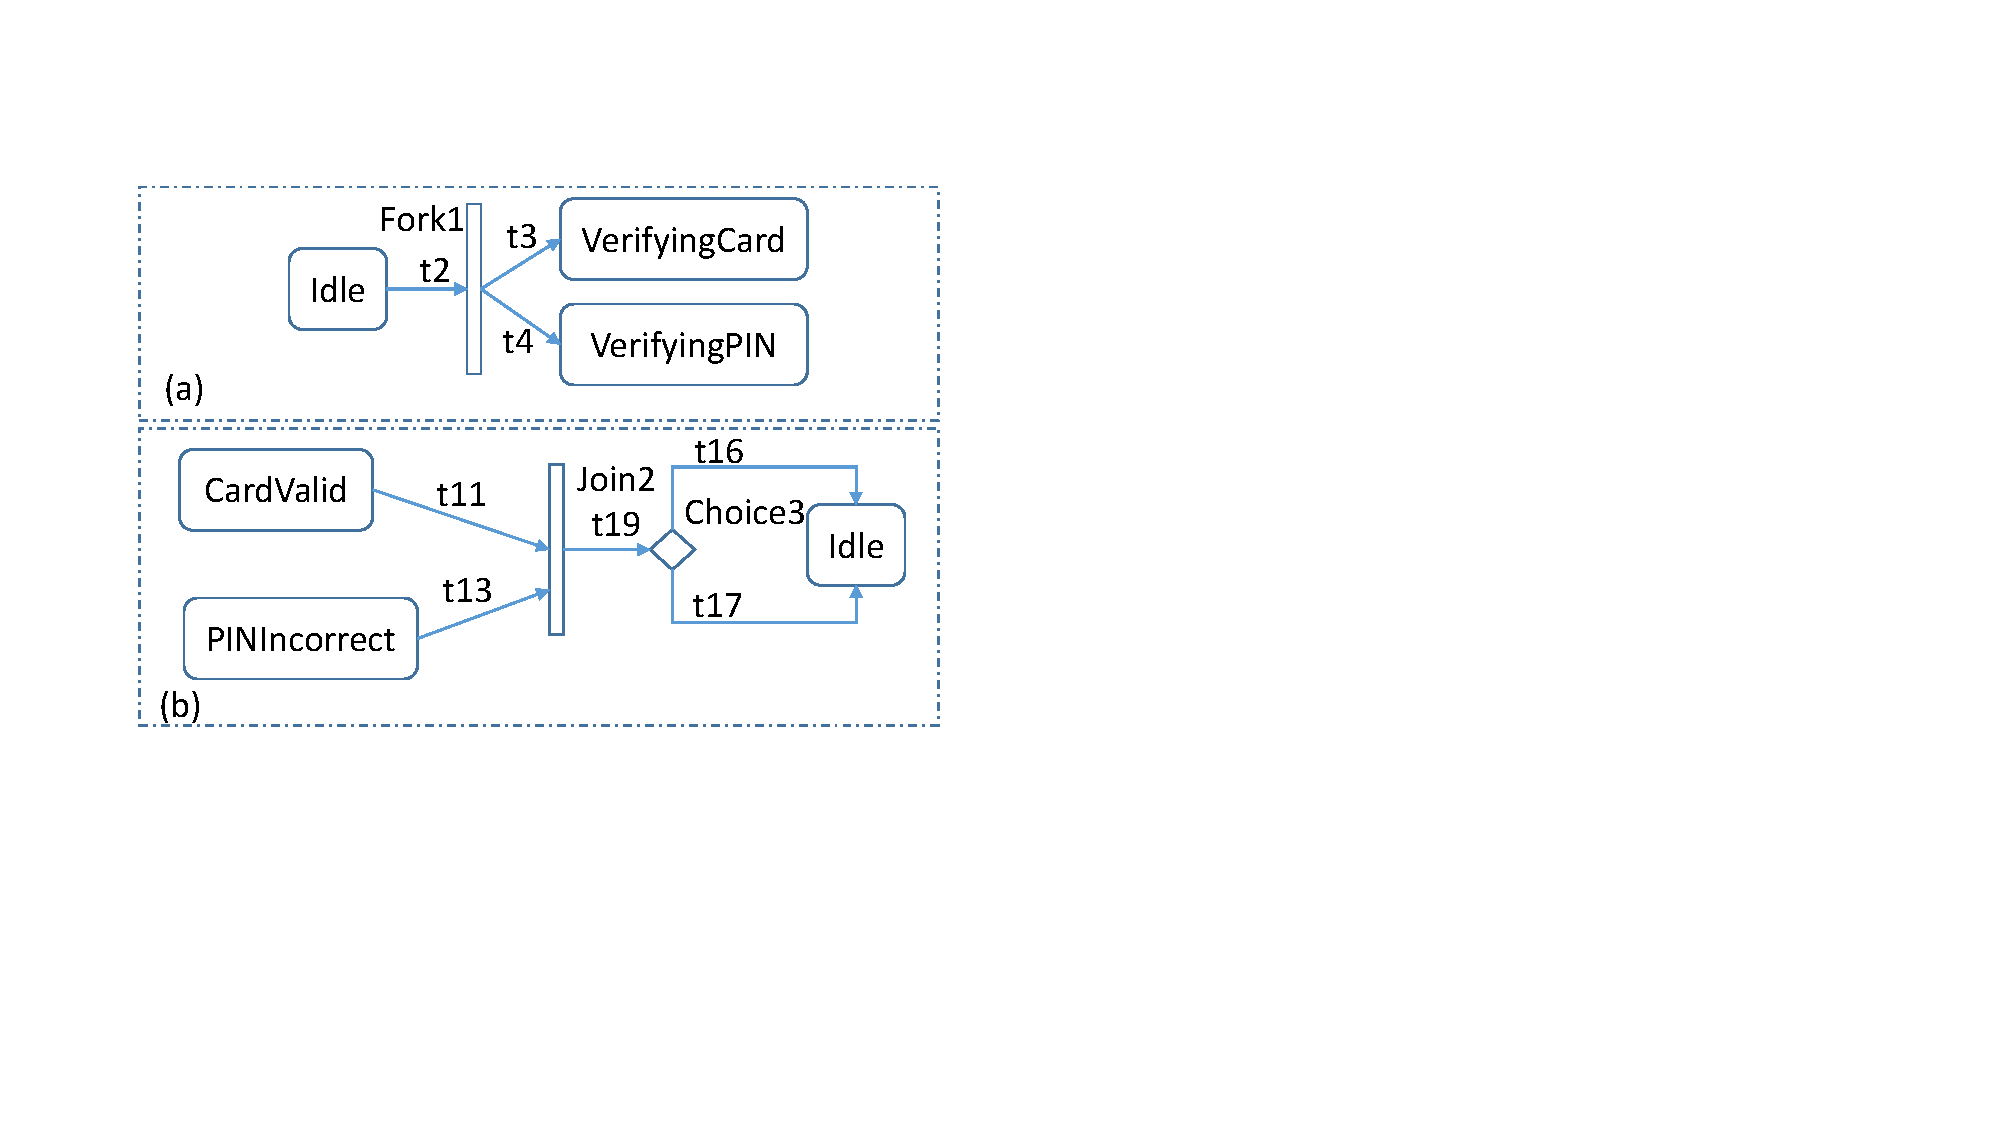
\includegraphics[clip, trim=2.0cm 6cm 17.5cm 3cm, width=\columnwidth]{figures/transitionGraph.pdf}
	\caption{Transition graphs} 
	\label{fig:transitionGraph}
\end{figure}


\begin{definition} A compound transition $t_{cp}$ is a virtual path which starts from one or multiple UML state and ends on one or multiple UML state. A compound transition is specified by a triple \{srcs($t_{cp}$), trc($t_{cp}$), tgts($t_{cp}$)\}, in which source part srcs($t_{cp}$) consists of one or multiple states, transition part trc($t_{cp}$) consists of multiple transitions, and target part tgts($t_{cp}$) consists of one or multiple states. 
\end{definition}


Given a state, Algorithm \ref{alg:cptransition} presents how to calculate transition graphs whose source $t_{cp}$ whose source part contains only a state $s$. 

\begin{algorithm}[]
	\caption{Transition graphs calculation
		\label{alg:cptransition}}
	\begin{algorithmic}[1]
		\Require{A state $s$ of a state machine}
		\Ensure{A set of transition graphs $\mathcal{GT}$}
		\Procedure{calculateTransGraphs}{$s$}
		\Let{$\mathcal{GT}$}{$\emptyset$} 
		\For {$out \in T_{outs}(s)$}
			\If {$tgt(out)$ is not a state}
				\Let{$\tau$}{($\mathcal{S}$, $\mathcal{L}$, $\mathcal{P}$, $\mathcal{T}$) $=\{\emptyset,\emptyset, \emptyset, \emptyset\}$}
				\Let{$\mathcal{P}$}{$\mathcal{P} \cup {tgt(out)}$}
				\Let{$\mathcal{S}$}{$\mathcal{S} \cup \{s\}$}
				\Let{$\mathcal{T}$}{$\mathcal{T} \cup {out}$}
				\If {$tgt(out).kind = join$}
					\Let{$ins$}{\\$\{i \in T_{ins}(tgt(out))| ctner(src(i)) = ctner(s)\}$}
					\Let{$\mathcal{S}$}{$\mathcal{S} \cup \{src(i)|i \in ins\}$}
					\Let{$\mathcal{T}$}{$\mathcal{T} \cup ins$}
				\EndIf
				\Let{$nexts$}{$FINDTRANS(tgt(out))$}
				\Let{$\mathcal{T}$}{$\mathcal{T} \cup nexts$}
				\Let{H}{\\$\{tgt(t)|t \in nexts \wedge tgt(t).kind = history\}$}
				\Let{$\mathcal{P}$}{$\mathcal{P} \cup \{src(t)|t \in nexts\} \cup H$}
				\Let{$\mathcal{L}$}{$\mathcal{L} \cup \{tgt(t)|t \in nexts \wedge tgt(t)$ is state $\}$}
								
				\Let{$\mathcal{GT}$}{$\mathcal{GT} \cup \{\tau\}$} 
			\EndIf
		\EndFor
		\EndProcedure
		
		\Require{A vertex $v$}
		\Ensure{Transition paths starting from $v$ and ending on a state}
		\Procedure{FindTrans}{$v$}
		\Let{$nextTrans$}{$T_{outs}(v)$}
		\For {$out \in T_{outs}(v)$}
			\If {$tgt(out)$ is not a state}
				\Let {$nextTrans$}{\\$nextTrans \cup FINDTRANS(tgt(out))$}
			\EndIf
		\EndFor	 			 	
		\Return {$nextTrans$} 
		\EndProcedure	
	\end{algorithmic}
\end{algorithm}

For example, applying this algorithm to all states of the state machine example in \ref{fig:example}, we can calculate other transition graphs which are:
\begin{IEEEeqnarray*}{lCr}
	\tau_{3} &=& (\mathcal{S}_3, \mathcal{L}_3, \mathcal{P}_3, \mathcal{T}_3) = (\{VerifyingCard\}, \{Idle, \\ 
	&& {} CardValid\}, \{Choice1\}, \{t5, t6, t7\}),
\end{IEEEeqnarray*}
\begin{IEEEeqnarray*}{lCr}	
	\tau_{4} &=& (\{VerifyingPIN\}, \{PINIncorrect, \\
	&& {} PINCorrect\}, \{Choice2\}, \{t8, t9, t10\}),
\end{IEEEeqnarray*} 
and
\begin{IEEEeqnarray*}{lCr}	
	\tau_{5} &=& (\{CardValid, PINCorrect\}, \{DispenseMoney\}, \\ 
	&& {} \{Join2\}, \{t12, t14, t15\}).
\end{IEEEeqnarray*} 

\end{comment}


\begin{definition} A transition graph $\tau$ is an acyclic directed graph ($\mathcal{T}_r$, $\mathcal{P}$, $\mathcal{T}$) where $\mathcal{P}$ is a set of vertexes, and $\mathcal{T}_{r}$ and $\mathcal{T}$ are sets of transitions. $\mathcal{T}_{r}$ is called the set of root transitions of the graph. Following conditions are satisfied:
	\begin{itemize}
		\item $\forall t \in \mathcal{T}_r, src(t)$ is a state.
		
		\item $\forall p \in \mathcal{P}, p.kind \notin \{state, composite, concurrent\}$.	
		
		\item $\forall t \in \mathcal{T}, src(t)$ is a pseudo state.
	\end{itemize}	
\end{definition}

A traversal from the root transitions of a transition graph to a stable state configuration is a compound transition. A state machine can contain multiple transition graphs. Fig. \ref{fig:transitionGraph} (a) and (b) show two transition graphs $\tau_{1}$ and $\tau_{2}$ of the ATM state machine, respectively, in which 
\begin{IEEEeqnarray*}{lCr}
	\tau_{1} &=& (\mathcal{T}_r, \mathcal{P}, \mathcal{T}) = (\{t2\}, \{Fork1\}, \{t3, t4\} )
\end{IEEEeqnarray*}
and
\begin{IEEEeqnarray*}{lCr}	
	\tau_{2} &=& (\{t11, t13\}, \{Join2, Choice3\}, \{t19, t16, t17\}).
\end{IEEEeqnarray*}



\begin{figure}
	\centering
	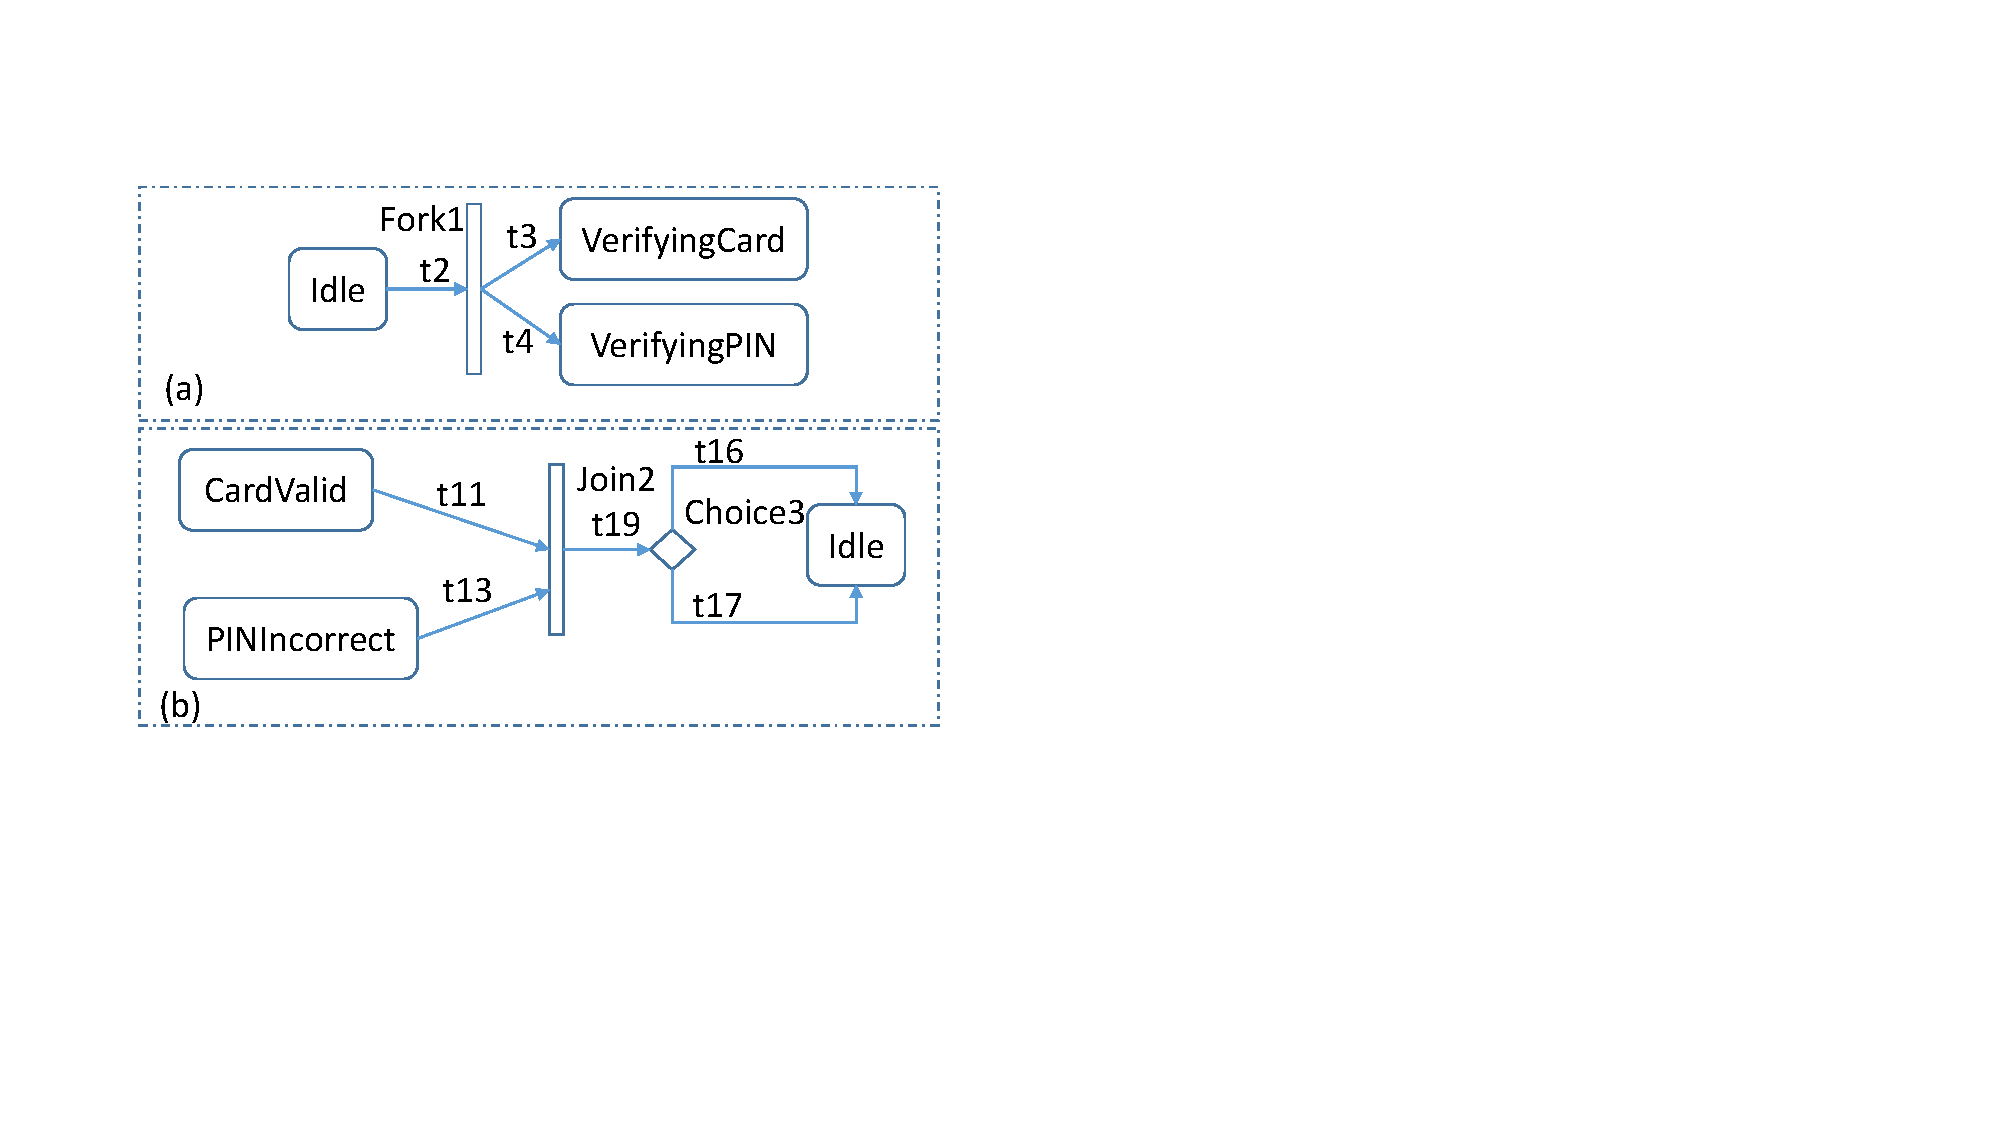
\includegraphics[clip, trim=2.0cm 6cm 17.5cm 3cm, width=\columnwidth]{figures/transitionGraph.pdf}
	\caption{Transition graphs} 
	\label{fig:transitionGraph}
\end{figure}

\begin{comment}
\begin{definition} A compound transition $t_{cp}$ is a virtual path which starts from one or multiple UML state and ends on one or multiple UML state. A compound transition is specified by a triple \{srcs($t_{cp}$), trc($t_{cp}$), tgts($t_{cp}$)\}, in which source part srcs($t_{cp}$) consists of one or multiple states, transition part trc($t_{cp}$) consists of multiple transitions, and target part tgts($t_{cp}$) consists of one or multiple states. 
\end{definition}
\end{comment}

Given a state, Algorithm \ref{alg:cptransition} presents how to calculate transition graph set whose root transitions outgo from $s$. 

\begin{algorithm}[]
	\caption{Transition graphs calculation
		\label{alg:cptransition}}
	\begin{algorithmic}[1]
		\Require{A state $s$ of a state machine}
		\Ensure{A set of transition graphs $\mathcal{GT}$}
		\Procedure{calculateTransGraphs}{$s$}
		\Let{$\mathcal{GT}$}{$\emptyset$} 
		\For {$out \in T_{outs}(s)$}
			\If {$tgt(out)$ is not a state}
				\Let{$\tau$}{($\mathcal{T}_r$, $\mathcal{P}$, $\mathcal{T}$) $=\{\emptyset,\emptyset, \emptyset\}$}
				\Let{$\mathcal{P}$}{$\mathcal{P} \cup {tgt(out)}$}
				\Let{$\mathcal{T}_r$}{$\mathcal{T}_r \cup {out}$}
			\If {$tgt(out).kind = join$} 
				\Let{$\mathcal{T}_r$}{$\mathcal{T}_r \cup T_{ins}(tgt(out))$}
			\EndIf
				\Let{$nexts$}{$FINDTRS(tgt(out))$}
				\Let{$\mathcal{T}$}{$\mathcal{T} \cup nexts$}
			
				\Let{$\mathcal{GT}$}{$\mathcal{GT} \cup \{\tau\}$} 
			\EndIf
		\EndFor
		\EndProcedure
		
		\Require{A vertex $v$}
		\Ensure{Transition paths starting from $v$ to atomic  states}
		\Procedure{FINDTRS}{$v$}
		\Let{$outs$}{$T_{outs}(v)$}
		\For {$out \in T_{outs}(v)$}
			\If {$tgt(out)$ is not a state}
				\Let {$outs$}{\\$outs \cup FINDTRS(tgt(out))$}
			\ElsIf $tgt(out).kind \in {composite, concurrent}$
				\For {$sub \in subvertexes(tgt(out)), sub.kind=initial$}
					\Let {$outs$}{$outs \cup FINDTRS(sub)$}
				\EndFor
			\EndIf 
		\EndFor	 			 	
		\Return {$outs$} 
		\EndProcedure	
	\end{algorithmic}
\end{algorithm}

For example, applying this algorithm to all states of the state machine example in \ref{fig:example}, we can calculate other transition graphs which are:
\begin{IEEEeqnarray*}{lCr}
	\tau_{3} &=& (\mathcal{S}_3, \mathcal{L}_3, \mathcal{P}_3, \mathcal{T}_3) = (\{VerifyingCard\}, \{Idle, \\ 
	&& {} CardValid\}, \{Choice1\}, \{t5, t6, t7\}),
\end{IEEEeqnarray*}
\begin{IEEEeqnarray*}{lCr}	
	\tau_{4} &=& (\{VerifyingPIN\}, \{PINIncorrect, \\
	&& {} PINCorrect\}, \{Choice2\}, \{t8, t9, t10\}),
\end{IEEEeqnarray*} 
and
\begin{IEEEeqnarray*}{lCr}	
	\tau_{5} &=& (\{CardValid, PINCorrect\}, \{DispenseMoney\}, \\ 
	&& {} \{Join2\}, \{t12, t14, t15\}).
\end{IEEEeqnarray*} 


\begin{definition} Current active configuration $Cfg$ of a UML state machine sm is a set of candidate UML states which are able to process an incoming event. 
\end{definition}

Given $sm$ is a flat state machine, whose vertex kinds are not in $\{composite, concurrent\}$, $\#Cfg (sm) = 1$ when the system (active class C) is running. 
$Cfg$ is also defined for composite/concurrent states. For each active composite/concurrent state $cs$, we write $subactives(cs)$ as a set of active sub-states of cs. If $cs.kind = composite$ then $\#subactives(cs) = 1$, otherwise $\#subactives(cs) > 1$. A transitive active set  $subactives^+$ of an active state $s$ is defined as following:

\begin{figure*}
	% ensure that we have normalsize text
	\normalsize
	% Store the current equation number.
	\setcounter{mytempeqncnt}{\value{equation}}
	% Set the equation number to one less than the one
	% desired for the first equation here.
	% The value here will have to changed if equations
	% are added or removed prior to the place these
	% equations are referenced in the main text.
	
	\begin{equation}
	subactives^+ (s) =    \left\{
	\begin{array}{ll}
	s & s.kind \notin \{composite, concurrent\}  \\
	\bigcup\limits_{sub \in subactives(s)} subactives^{+} (sub) & s.kind \in \{composite, concurrent\} \\
	\end{array} 
	\right. 
	\end{equation}
	% Restore the current equation number.
	\setcounter{equation}{\value{mytempeqncnt}}
	% IEEE uses as a separator
	%\hrulefill
	% The spacer can be tweaked to stop underfull vboxes.
	%\vspace*{4pt}
\end{figure*}

	


Therefore, we write:
\begin{equation}
	Cfg(sm) = subactives^+(subactives(sm))
\end{equation}

\subsection{Event dispatching}
An external event incoming to the system or an internal event emitted by the system is dispatched by checking whether the innermost active states accept the event or not. Algorithm \ref{alg:event-processing}, in which $isAccepted(s, e)$ is $true$ if the event $e$ is accepted by the state $s$, shows how an event should be dispatched by the system.  

\begin{algorithm}[]
	\caption{Event dispatching
		\label{alg:event-processing}}
	\begin{algorithmic}[1]
		\Require{An incomming event e, active state s\_active of the running state machine sm}
		\Ensure{Event is processed}
		\Procedure{dispatchEvent}{$s\_active$, $e$}
		\Let{$ret$}{$false$}
		\If {$s\_active.kind \in {composite, concurrent}$}
			\For {$sub \in subactives(s_active)$}
				\State{@concurrentExec \\ $(ret = DISPATCHEVENT(sub, e) \vee ret)$}
			\EndFor	 			 
		\EndIf
		\State{\ti{Wait for all cocurrent executions terminate}}
		\If {$(s\_active.kind = state) \vee !ret$}
			\If {$isAccepted(s\_active)$}
				\Let{$ret$}{$true$}
				\State $processEvent(s\_active, e)$
			\EndIf
		\EndIf
		\Return{ret} 
		\EndProcedure	
	\end{algorithmic}
\end{algorithm}

In Algorithm \ref{alg:event-processing}, if the active state of the state machine $sm$ is atomic, a $processEvent$ procedure is executed to transition the active state to another state. Otherwise said, the active state delegates the event processing to its active sub-state. If the event is not consumed by the active sub-state, the processing of the former is delegated back to the parent state of the latter. In the following section, we show how to change the active state of the state machine.


\subsection{Event processing semantics}
There are three ways of transitioning from one state to another state including (1) direct transitioning in which the source state is directly connected to the target state by a transition, and (2) indirect transitioning in which multiple transitions and pseudo states in a transition graph are involved.

\subsubsection{Direct transition}
An active state can be changed from a source state to a target state either within the same region or not. In the first case, the transition $t$ connecting the two states is in the same region. This case is simply that the source state ends its activity and all of its active sub-states. In the second case, given a source state $s_{src}$, a target state $s_{tgt}$, and the transition $t$ connecting the two states, the following sub-cases are differentiated:
\begin{itemize}
	\item $s_{src} = ctner(s_{tgt}) \vee s_{src} \in ctner^+(s_{tgt})$
	
	\item $s_{tgt} = ctner(s_{src}) \vee s_{tgt} \in ctner^+(s_{src})$
	
	\item $s_{src} = s_{tgt}$
	
%	\item $ctner(s_{src}) \in ctner^+(s_{tgt})$
	
%	\item $ctner(s_{tgt}) \in ctner^+(s_{src})$
	
	\item $\exists s_{src}^* \in ctner^+(s_{src}) \wedge \exists s_{tgt}^* \in ctner^+(s_{tgt}): ctner(s_{src}^*) = ctner(s_{tgt}^*)$.
\end{itemize}  

The first and second sub-cases are occurred when the transition lies between a composite state and one of its transitive sub-states. The transition execution depends on the kind of $t$ which is either local or external. The third sub-case is a special case in which only the transition effect is executed. Algorithm \ref{alg:transition1} shows the execution order of these three sub-cases. 

\begin{algorithm}[]
	\caption{Transition Execution 1
		\label{alg:transition1}}
	\begin{algorithmic}[1]
		\Require{A transition $t$ with its source and target states as $s_{src}$ and $s_{tgt}$}
		\Ensure{Transition is correctly executed}
		\Procedure{executeTrans}{$t$, $s_{src}$, $s_{tgt}$}
		\Let{$ret$}{$false$}
		\If {$s\_active.kind \in {composite, concurrent}$}
		\For {$sub \in subactives(s_active)$}
		\State{@concurrentExec \\ $(ret = DISPATCHEVENT(sub, e) \vee ret)$}
		\EndFor	 			 
		\EndIf
		\State{\ti{Wait for all cocurrent executions terminate}}
		\If {$(s\_active.kind = state) \vee !ret$}
		\If {$isAccepted(s\_active)$}
		\Let{$ret$}{$true$}
		\State $processEvent(s\_active, e)$
		\EndIf
		\EndIf
		\Return{ret} 
		\EndProcedure	
	\end{algorithmic}
\end{algorithm}

\subsubsection{Indirect transition}